\documentclass[a4paper, 11pt, titlepage]{article}
\usepackage[utf8]{inputenc}
\usepackage[english]{babel}
\usepackage[]{parskip}
\usepackage{graphicx}
\usepackage{xcolor}
\usepackage{paralist} % compactitem
\usepackage{csquotes}
\usepackage{wrapfig}
\usepackage{subfig}
\usepackage{csvsimple}
% Citations
\usepackage[
  style=ieee,
  citecounter,
  labelnumber,
  backend=biber,
  bibencoding=utf8,
  sorting=none
]{biblatex}
\addbibresource{references.bib}
% Code blocks
\usepackage{listings}
\definecolor{codegreen}{rgb}{0,0.6,0}
\definecolor{codegray}{rgb}{0.5,0.5,0.5}
\definecolor{codepurple}{rgb}{0.58,0,0.82}
\definecolor{backcolour}{rgb}{1.0,1.0,1.0}
\lstdefinestyle{mystyle}{
  backgroundcolor=\color{backcolour},
  commentstyle=\color{codegreen},
  keywordstyle=\color{magenta},
  numberstyle=\tiny\color{codegray},
  stringstyle=\color{codepurple},
  basicstyle=\ttfamily\tiny,
  breakatwhitespace=false,
  breaklines=true,
  captionpos=b,
  keepspaces=false,
  numbersep=5pt,
  showspaces=false,
  showstringspaces=false,
  showtabs=false,
  tabsize=2
}
\lstset{style=mystyle}
% Custom commands
\newcommand{\figRef}[1]{Figure \ref{#1}}
\newcommand{\tabRef}[1]{Table \ref{#1}}
\newcommand{\eqRef}[1]{(\ref{#1})}

\title{EECE6036 - Homework 2}
\author{Wayne Stegner}
\date{\today}

\begin{document}
  \maketitle
  \section{Problem 1}
  \subsection{Problem Summary}
  \subsection{Results}
  \begin{figure}[ht]
    \center
    \subfloat[]{
      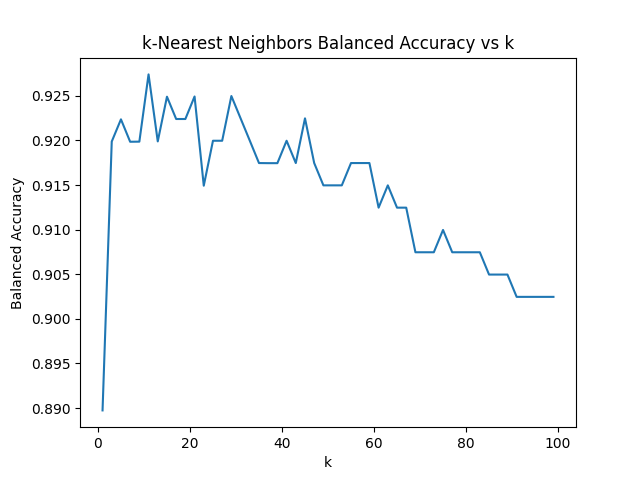
\includegraphics[width=0.47\textwidth]{images/knn_bal_acc.png}
      \label{fig:knn_bal_acc}
    }
    \subfloat[]{
      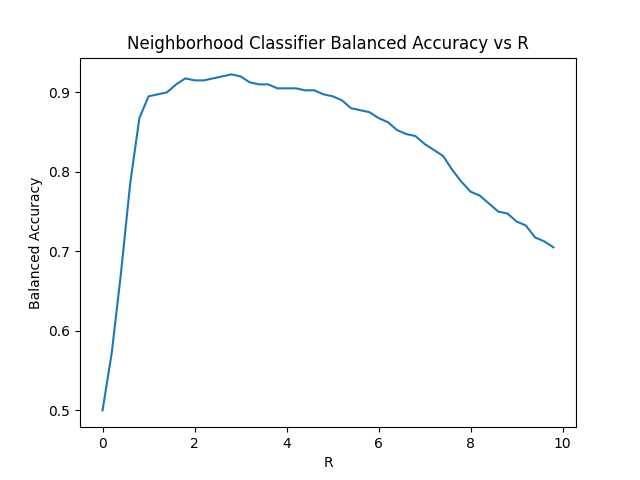
\includegraphics[width=0.47\textwidth]{images/neighborhood_bal_acc.png}
      \label{fig:neighborhood_bal_acc}
    }
    \caption{Balanced accuracy for KNN (a) and Neighborhood Classifier (b).}
    \label{fig:neighbor_bal_acc}
  \end{figure}
  \subsection{Discussion}
  \subsection{Conclusion}
  \pagebreak
  \section{Problem 2}
  \subsection{Problem Summary}
  \subsection{Results}
  \begin{figure}[ht]
    \center
    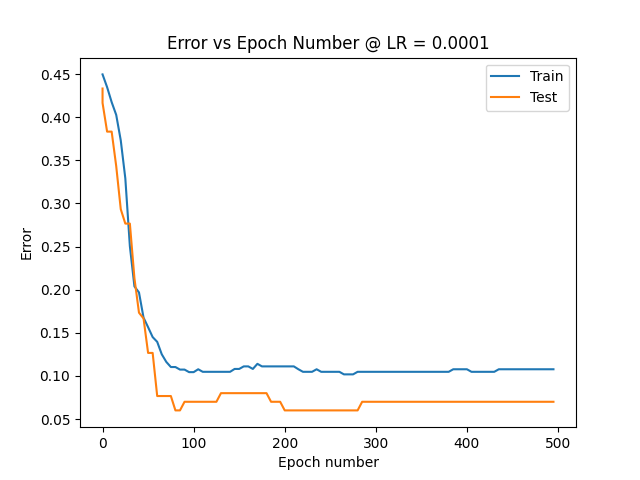
\includegraphics[width=0.47\textwidth]{images/perceptron_err.png}
    \caption{Training and testing error for a single perceptron.}
    \label{fig:perceptron_error}
  \end{figure}
  \subsection{Discussion}
  \subsection{Conclusion}
  \pagebreak
  \section{Problem 3}
  \subsection{Problem Summary}
  \subsection{Results}
  \subsubsection{Performance on Individual Trials}
  \par 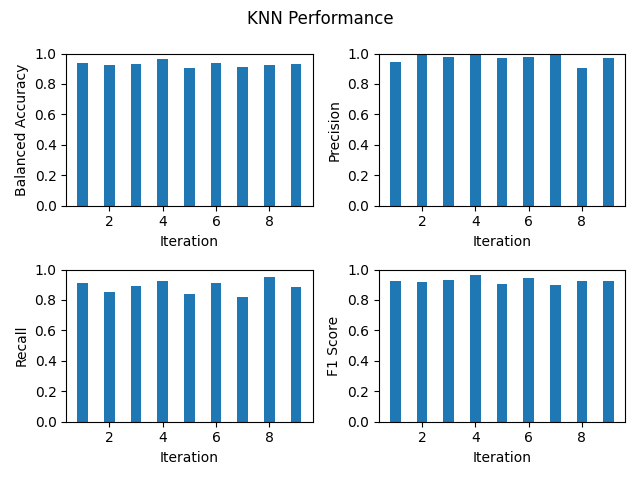
\includegraphics[width=0.85\textwidth]{images/knn_performance.png}
  \par 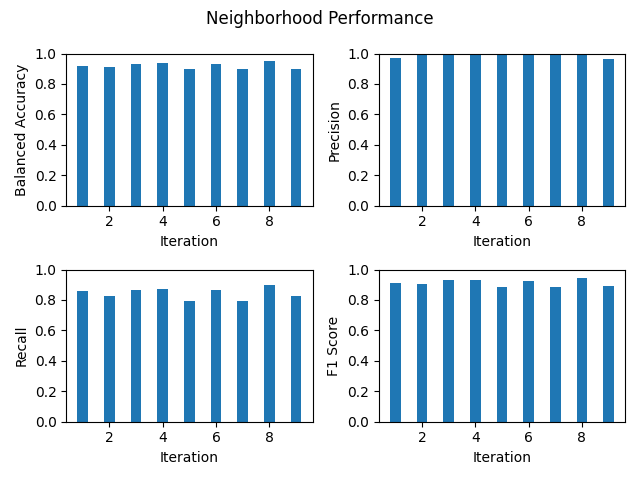
\includegraphics[width=0.85\textwidth]{images/neighborhood_performance.png}
  \par 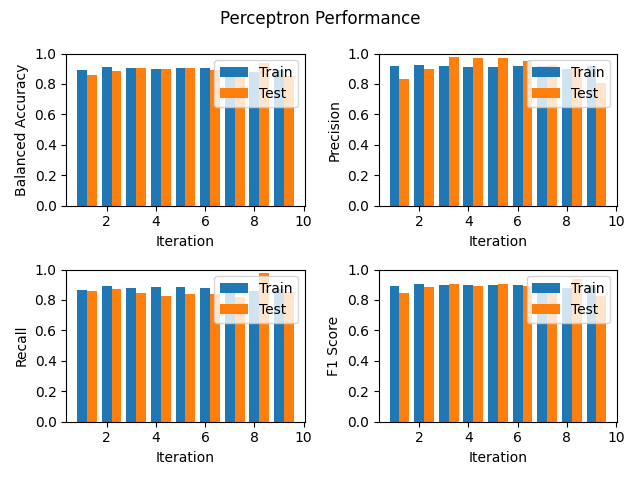
\includegraphics[width=0.85\textwidth]{images/perceptron_performance.png}
  \subsubsection{Average Performance}
  \begin{table}[h]
    \caption{Average performance of the classifiers.}
    \begin{center}
      \csvautotabular{data/avg_perf.csv}
    \end{center}
    \label{tab:avg_perf}
  \end{table}
  \subsubsection{Trial-Wise Training Error for the Perceptrons}
  \par 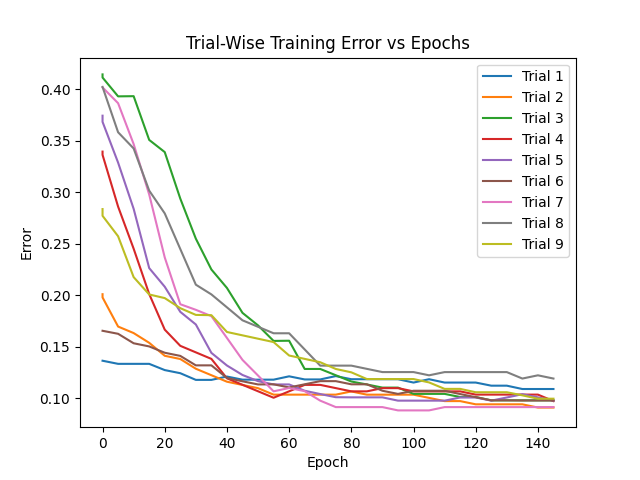
\includegraphics[width=0.85\textwidth]{images/trial_wise_error.png}
  \subsubsection{Mean Training Error for the Perceptron}
  \par 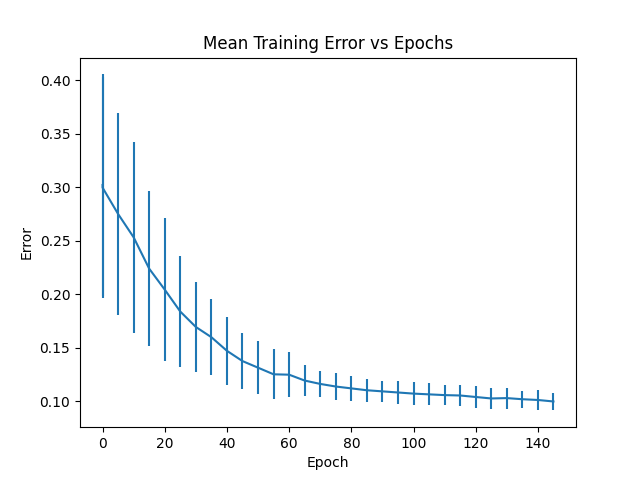
\includegraphics[width=0.85\textwidth]{images/mean_error.png}
  \subsubsection{Best KNN Decision Boundary}
  \par 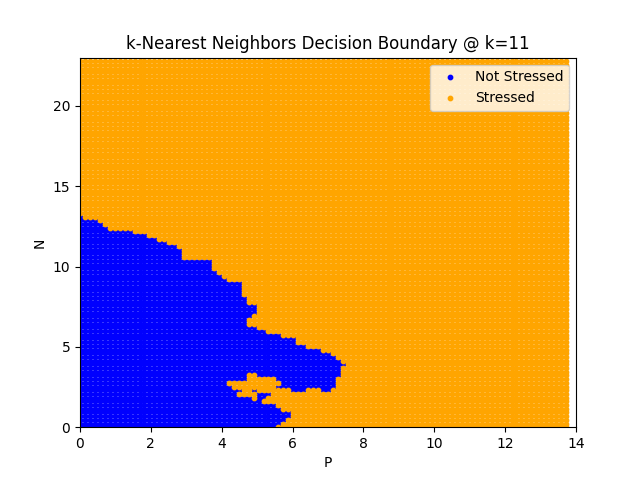
\includegraphics[width=0.85\textwidth]{images/knn_dec_bound.png}
  \subsubsection{Best Neighborhood Classifier Decision Boundary}
  \par 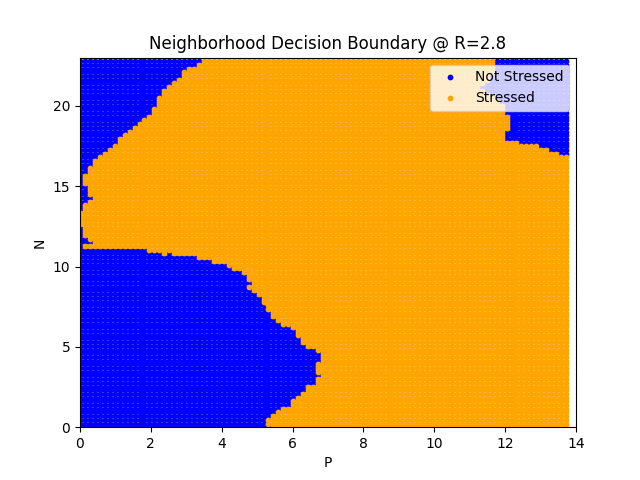
\includegraphics[width=0.85\textwidth]{images/neighborhood_dec_bound.png}
  \subsubsection{Perceptron Decision Boundary}
  \par 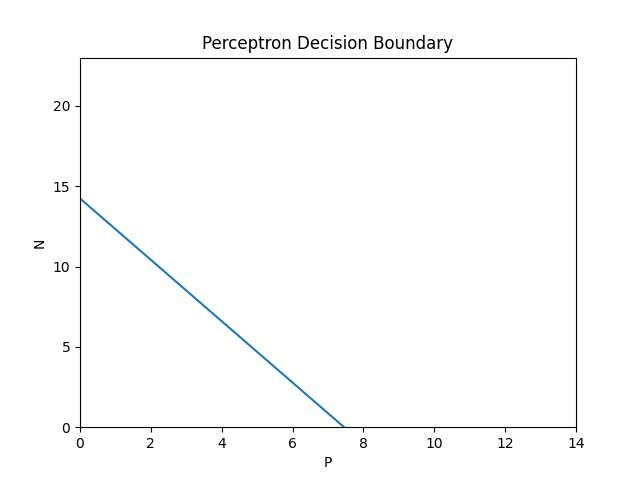
\includegraphics[width=0.85\textwidth]{images/perceptron_dec_bound.png}
  \subsubsection{Analysis of Results}
  \subsection{Discussion}
  \subsection{Conclusion}
  \pagebreak
  \appendix
  \section{Code}
  \subsection{\texttt{dataset.py}}
  \lstinputlisting[language=python]{"code/dataset.py"}
  \subsection{\texttt{classifier.py}}
  \lstinputlisting[language=python]{"code/classifier.py"}
  \subsection{\texttt{knn.py}}
  \lstinputlisting[language=python]{"code/knn.py"}
  \subsection{\texttt{neighborhood.py}}
  \lstinputlisting[language=python]{"code/neighborhood.py"}
  \subsection{\texttt{perceptron.py}}
  \lstinputlisting[language=python]{"code/perceptron.py"}
  \subsection{\texttt{problem\_3.py}}
  \lstinputlisting[language=python]{"code/problem_3.py"}
\end{document}
